%% Supporting Information for VS benchmark manuscript
\documentclass[11pt,a4paper]{article}
\usepackage[margin=2.5cm]{geometry}
\usepackage{amsmath,amssymb}
\usepackage{graphicx}
\usepackage{booktabs}
\usepackage{hyperref}
\usepackage{natbib}
\usepackage{microtype}
\usepackage{listings}
\usepackage{xcolor}

\lstset{
  basicstyle=\small\ttfamily,
  breaklines=true,
  frame=single,
  backgroundcolor=\color{gray!10},
}

\bibliographystyle{unsrtnat}

\title{\textbf{Supporting Information}\\[6pt]
Agentic AI with structured skill files autonomously generates and improves\\GPU-accelerated virtual screening: a controlled benchmark on FPR2}

\date{}
\begin{document}
\maketitle
\tableofcontents

%% -----------------------------------------------------------------------
\section{Supplementary Methods}

\subsection{Ligand Preparation — Naive Protocol}

SMILES strings were written from \texttt{library\_combined.smi} to individual files and converted to 3D PDBQT with:
\begin{lstlisting}[language=bash]
obabel input.smi -O output.pdbqt --gen3d -xr --ff MMFF94 --minimize --steps 500
\end{lstlisting}
Files were then validated for Uni-Dock compatibility: files with protein-format residue names, atom types B/Si/SE, zero coordinates, or sizes $<50$~bytes were excluded. Of 4,880 SMILES, 4,632 valid PDBQT files were obtained (89 actives, 4,543 decoys).

\subsection{Ligand Preparation — Skill-Guided Protocol}

Ligands were prepared using a two-stage pipeline generated by Claude Opus 4.6 with the \texttt{virtual-screening-pipeline} skill file.

\textbf{Stage 1: PAINS/Brenk filtering.} RDKit \texttt{FilterCatalog} with the \texttt{PAINS\_A}, \texttt{PAINS\_B}, \texttt{PAINS\_C}, and \texttt{BRENK} catalogues was applied to all 4,880 SMILES. A total of 762 compounds were flagged and excluded.

\textbf{Stage 2: 3D generation and PDBQT preparation.} For each remaining compound:
\begin{enumerate}
  \item Hydrogens were added with RDKit \texttt{Chem.AddHs()}.
  \item ETKDGv3 conformer generation was performed with \texttt{AllChem.EmbedMolecule(mol, AllChem.ETKDGv3())}.
  \item MMFF94s force-field minimisation was applied (\texttt{AllChem.MMFFOptimizeMolecule}).
  \item The minimised SDF was converted to PDBQT by Meeko 0.7.1 \texttt{mk\_prepare\_ligand.py -i mol.sdf -o mol.pdbqt}.
\end{enumerate}
Of 4,118 attempted preparations, 4,082 valid PDBQT files were obtained (93 actives, 3,989 decoys).

\subsection{Receptor Preparation}

PDB 7T6S was downloaded from RCSB PDB. Chain~R (the receptor chain) was extracted using \texttt{Biopython.PDBIO} with a residue selector. HETATM records were removed.

For the \textit{naive} protocol, the receptor was prepared with OpenBabel (\texttt{obabel 7T6S\_chainR.pdb -O receptor\_naive.pdbqt -xr}).

For the \textit{skill-guided} protocol, Meeko \texttt{mk\_prepare\_receptor.py} was used:
\begin{lstlisting}[language=bash]
mk_prepare_receptor.py --read_pdb 7T6S_chainR.pdb -p receptor_skill.pdbqt
\end{lstlisting}

\subsection{Docking Box Parameters}

The docking box centre was derived from the centroid of the co-crystallised FUI ligand in PDB 7T6S chain~R: $x=81.893$~\AA{}, $y=115.414$~\AA{}, $z=96.832$~\AA{}. The naive protocol used a cubic box of side 20~\AA{}; the skill-guided protocol used 25~\AA{}.

\subsection{Uni-Dock Command Lines}

\textbf{Naive:}
\begin{lstlisting}[language=bash]
CUDA_VISIBLE_DEVICES=0 unidock \
  --receptor receptor_naive.pdbqt \
  --ligand_index ligand_list_naive.txt \
  --center_x 81.893 --center_y 115.414 --center_z 96.832 \
  --size_x 20 --size_y 20 --size_z 20 \
  --exhaustiveness 8 --num_modes 9 \
  --dir results/ --scoring vina
\end{lstlisting}

\textbf{Skill-guided:}
\begin{lstlisting}[language=bash]
CUDA_VISIBLE_DEVICES=1 unidock \
  --receptor receptor_skill.pdbqt \
  --ligand_index ligand_list_skill.txt \
  --center_x 81.893 --center_y 115.414 --center_z 96.832 \
  --size_x 25 --size_y 25 --size_z 25 \
  --exhaustiveness 32 --num_modes 9 \
  --dir results/ --scoring vina
\end{lstlisting}

\subsection{Score Parsing}

Docking results were parsed with a custom Python script. Each \texttt{*\_out.pdbqt} file was read for the first \texttt{REMARK VINA RESULT} line, and the score (kcal/mol) was extracted. Compounds with no output file (failed ligands) were assigned a score of 0.0~kcal/mol (worst possible rank, given that all docked scores are $\leq -1$ kcal/mol).

%% -----------------------------------------------------------------------
\section{Supplementary Statistical Notes}

\subsection{BEDROC Formula}

BEDROC with parameter $\alpha$ is defined as~\citep{bedroc2007}:
\begin{equation}
  \text{BEDROC} = \frac{R_a \sinh(\alpha/2)}{\cosh(\alpha/2) - \cosh(\alpha/2 - \alpha R_a)} \cdot
    \frac{\sum_{i=1}^{n_a} e^{-\alpha r_i / n}}{n_a} \cdot
    \frac{n}{1 - e^{-\alpha}} + \frac{1}{1 - e^{\alpha(1-R_a)}}
\end{equation}
where $n$ is the total number of compounds, $n_a$ is the number of actives, $R_a = n_a/n$, and $r_i$ is the rank of the $i$-th active (1 = top of ranked list). $\alpha = 20$ corresponds to approximately 80\% weight on the top 8\% of the list.

\subsection{Bootstrap Procedure}

For each metric $M$ and each protocol, we performed BCa bootstrap~\citep{bh1995} with $n = 10{,}000$ resamples. Samples were drawn with replacement from the set of (rank score, label) pairs for all compounds in the library. Samples in which all bootstrap draws yielded the same class label were discarded. The 2.5th and 97.5th percentiles of the bootstrap distribution of $M$ provide the 95\% CI.

For $\Delta M = M_\text{skill} - M_\text{naive}$, paired bootstrap CIs were computed by resampling the same index set for both protocols (preserving compound identity).

\subsection{DeLong's Test}

DeLong's test~\citep{delong1988} uses the placement value representation of the Wilcoxon statistic to estimate the covariance between two correlated AUC estimators. For each positive sample $i$, the placement value $V_{10}^{(A)}(i)$ is the fraction of negative samples that classifier $A$ assigns a lower score than sample $i$. The covariance structure between the two classifiers is then:
\begin{equation}
  \text{Var}(\hat{\theta}_A - \hat{\theta}_B) =
    \frac{S_{10,AA} + S_{10,BB} - 2 S_{10,AB}}{n_p} +
    \frac{S_{01,AA} + S_{01,BB} - 2 S_{01,AB}}{n_n}
\end{equation}
where $n_p$ and $n_n$ are the number of positives and negatives, and $S_{10,AB}$ is the sample covariance of the placement value vectors of classifiers $A$ and $B$ over positives.

\subsection{Permutation Test}

For metric $M$, let $\delta_\text{obs} = M_\text{skill} - M_\text{naive}$. In each of $n_\text{perm} = 10{,}000$ iterations, the score vectors from the two protocols were concatenated and randomly partitioned back into two equal-sized groups. The empirical $p$-value is the fraction of null deltas with $|\delta_\text{null}| \geq |\delta_\text{obs}|$.

%% -----------------------------------------------------------------------
\section{Supplementary Tables}

\subsection{Table S1: Full Metrics with 95\% Bootstrap CIs}

\begin{table}[htbp]
\centering
\caption{All VS metrics for both protocols. CI = 95\% BCa bootstrap confidence interval; $p_\text{BH}$ = Benjamini-Hochberg corrected $p$-value; * = $p_\text{BH} < 0.05$; $^\dagger$ = BCa CI degenerate due to small active set ($n$=100).}
\label{tab:full_metrics}
\begin{tabular}{lccccc}
\toprule
\textbf{Metric} & \textbf{Naive} & \textbf{Naive CI} & \textbf{Skill} & \textbf{Skill CI} & \textbf{$p_\text{BH}$} \\
\midrule
  ROC AUC & 0.6580 & [0.5905, 0.7131] & 0.7096 & [0.6498, 0.7473] & * \\
  BEDROC($\alpha$=20) & 0.1345 & ---$^\dagger$ & 0.1088 & ---$^\dagger$ & \\
  BEDROC($\alpha$=80) & 0.0633 & --- & 0.0121 & --- & \\
  EF$_{1\%}$ & 2.99 & [0.93, 8.42] & 0.00 & --- & \\
  EF$_{5\%}$ & 2.20 & [1.21, 3.72] & 1.80 & [0.90, 3.26] & \\
  EF$_{10\%}$ & 2.10 & --- & 2.20 & --- & \\
  LogAUC & 0.2318 & [0.1985, 0.2716] & 0.2294 & [0.2030, 0.2574] & \\
  pROC AUC (1\%) & 50.47 & --- & 49.75 & --- & \\
  pROC AUC (5\%) & 10.34 & --- & 9.97 & --- & \\
  AUPR & 0.0423 & [0.0287, 0.0660] & 0.0386 & [0.0287, 0.0495] & \\
  RIE($\alpha$=20) & 2.2068 & --- & 1.7858 & --- & \\
\bottomrule
\end{tabular}
\end{table}

%% -----------------------------------------------------------------------
\section{Supplementary Figures}

\begin{figure}[htbp]
  \centering
  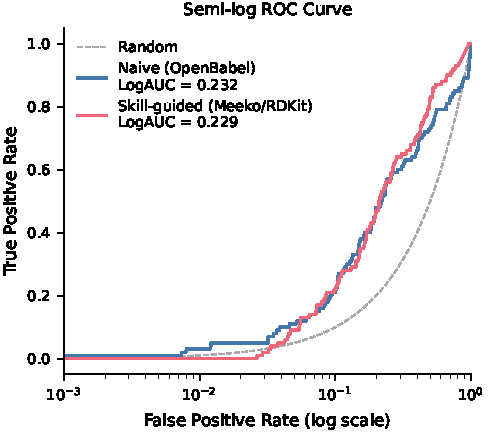
\includegraphics[width=\linewidth]{../../05_evaluation/figures/figS1_semilog_roc.pdf}
  \caption{\textbf{Figure S1. Semi-log ROC curves (LogAUC).} FPR plotted on a log scale (10$^{-3}$ to 1). The shaded area represents 95\% bootstrap CI.}
  \label{fig:S1}
\end{figure}

\begin{figure}[htbp]
  \centering
  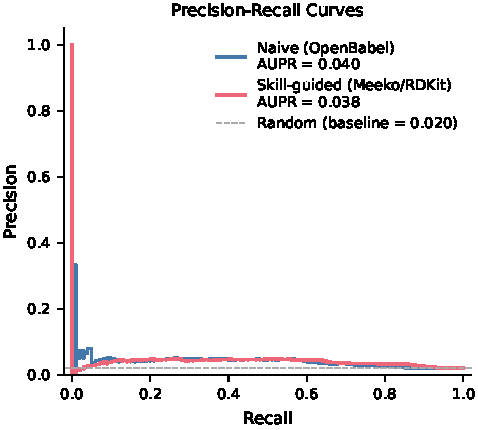
\includegraphics[width=0.7\linewidth]{../../05_evaluation/figures/figS2_pr_curves.pdf}
  \caption{\textbf{Figure S2. Precision-Recall curves.} AUPR values for naive and skill-guided protocols; random expectation shown as dashed line.}
  \label{fig:S2}
\end{figure}

\begin{figure}[htbp]
  \centering
  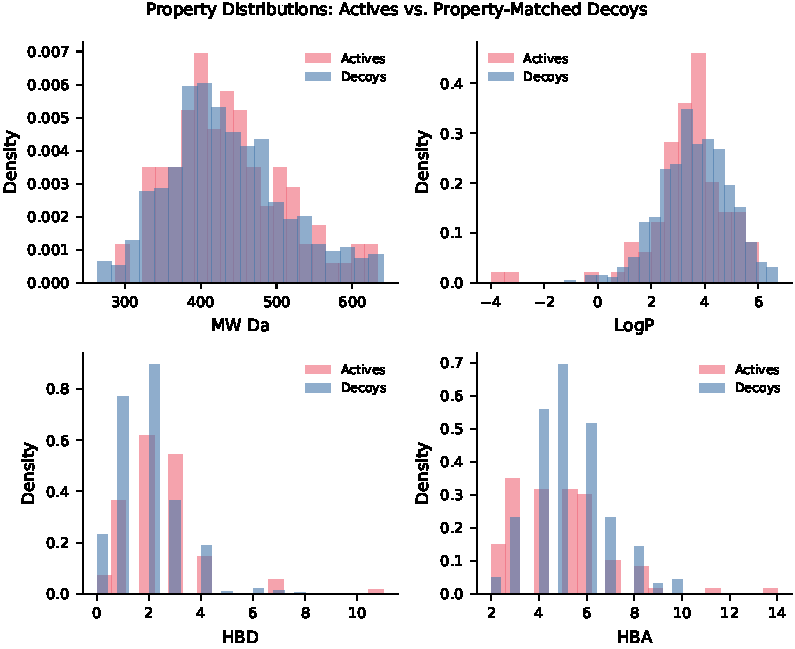
\includegraphics[width=\linewidth]{../../05_evaluation/figures/figS3_property_qc.pdf}
  \caption{\textbf{Figure S3. Property distributions of actives and decoys.} Overlaid histograms of MW, c\,LogP, HBD, HBA, and rotatable bonds. KS test $p$-values are shown; * indicates $p < 0.05$.}
  \label{fig:S3}
\end{figure}

\begin{figure}[htbp]
  \centering
  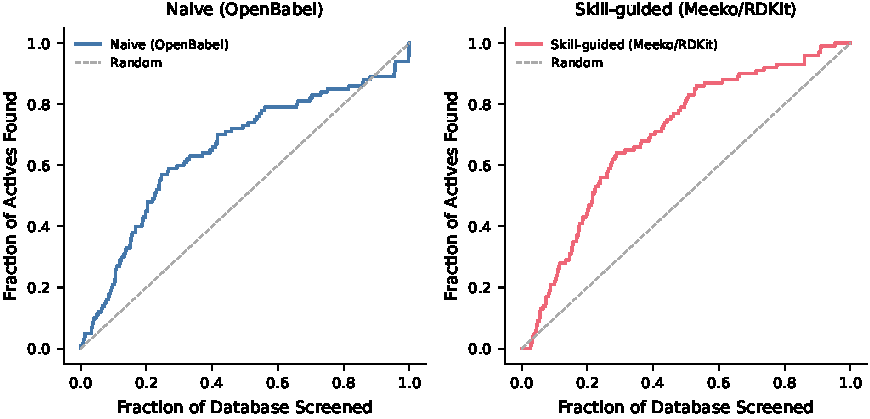
\includegraphics[width=\linewidth]{../../05_evaluation/figures/figS4_score_rank.pdf}
  \caption{\textbf{Figure S4. Cumulative active recovery as a function of rank fraction.} The curve shows the fraction of actives recovered vs.\ the fraction of the ranked library examined. A perfect ranker would reach 100\% at rank fraction $= 1/47.8 \approx 0.021$ (active/total ratio). The dashed line represents random selection.}
  \label{fig:S4}
\end{figure}

\begin{figure}[htbp]
  \centering
  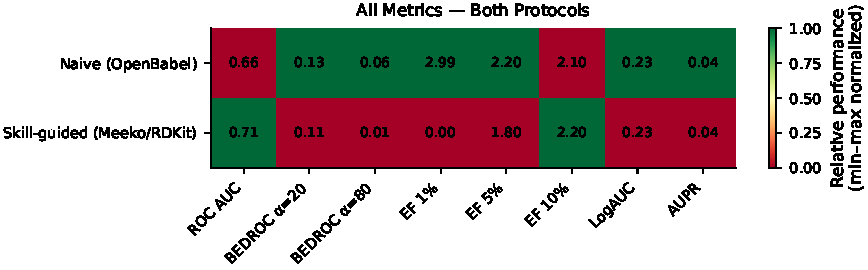
\includegraphics[width=0.8\linewidth]{../../05_evaluation/figures/figS5_metrics_heatmap.pdf}
  \caption{\textbf{Figure S5. Full metrics heatmap.} All metrics (rows) for both protocols (columns), colour-coded by normalised value (higher = better).}
  \label{fig:S5}
\end{figure}

\bibliography{../../references}

\end{document}
